\documentclass[sigconf]{acmart}

\settopmatter{printacmref=false}
\renewcommand\footnotetextcopyrightpermission[1]{}
\pagestyle{plain}

% Additional packages
\usepackage{listings}
\usepackage{algorithm}
\usepackage{algorithmic}
\usepackage{subcaption}
\usepackage{multirow}
\usepackage{array}
\usepackage{balance}
\usepackage{cleveref}
\usepackage[utf8]{inputenc}
\usepackage{xurl}

% Configure listings for Terraform code
\lstset{
    basicstyle=\footnotesize\ttfamily,
    breaklines=true,
    captionpos=b,
    frame=tb,
    numbers=left,
    numberstyle=\tiny\color{gray},
    showstringspaces=false,
    tabsize=2,
    commentstyle=\color{gray!70},
    keywordstyle=\color{blue!80!black},
    stringstyle=\color{red!70!black},
    backgroundcolor=\color{gray!5}
}

% Custom commands for consistency
\newcommand{\tool}[1]{\textsc{#1}}
\newcommand{\code}[1]{\texttt{#1}}
\newcommand{\file}[1]{\texttt{#1}}

% Graphics path
\graphicspath{{images/}}

\begin{document}

% Title and author information
\title{When AI Meets Terraform: A Reality Check on Code Generation for Infrastructure-as-Code}

\author{Lukas Buck}
\affiliation{%
  \institution{Reutlingen University - Faculty of Computer Science}
  \streetaddress{Street Address}
  \city{Reutlingen,} 
  \state{\texttt{Baden-Württemberg}}
  \country{Germany}
  \postcode{Postal Code}
}
\email{Lukas.Buck@Student.Reutlingen-University.de}

% Abstract
\begin{abstract}
Infrastructure-as-Code (IaC) has become indispensable for managing cloud resources, with Terraform emerging as the leading language for configuring such systems. While AI-powered coding assistants promise to accelerate development through code generation, their effectiveness for specialised domains such as IaC remains largely unexplored. This study presents a systematic evaluation of AI coding tools for Terraform development, comparing GitHub Copilot and Windsurf across 66 executions.


We designed 11 representative Terraform tasks ranging from simple resource provisioning to complex multi-layered architectures, and ran each scenario three times per tool to evaluate both performance and consistency. Our evaluation framework measured functionality, completeness, and code quality. The respective values were then rated with numbers, with a maximum total score of 6 points.

The results show significant differences in the capabilities of Copilot and Windsurf for IaC tasks. Copilot achieved an average score of 4.06 and Windsurf a score of 5.91. Windsurf remained very consistent across all tasks in terms of evaluation ($\sigma$ = 0.32), while Copilot showed great variance and quality ($\sigma$ = 1.35) in different implementations and tasks. However, both tools scored well with functioning code; only 3\% of the code written by Windsurf contained syntactic errors, while Copilot had no syntactic errors at all. On the other hand, there was a clear difference in the speed at which the AI assistants solved the tasks. Windsurf solved the tasks in an average of 75.1 seconds, while Copilot solved them in 29.2 seconds.

Our results show that there are already promising AI tools available for implementing IaC projects, but further development and improvements are needed to ensure that developers can truly rely on the assistant. The study provides practical guidelines for developers and sets benchmarks for future research in the field of IaC automation. All experimental data and generated configurations are publicly available for reproducibility.

\end{abstract}

% CCS concepts
\ccsdesc[500]{Computing methodologies~Artificial intelligence}
\ccsdesc[300]{Software and its engineering~Software development process tools}  
\ccsdesc[300]{Software and its engineering~Software testing and debugging}
\ccsdesc[100]{Computer systems organization~Cloud computing}

% Keywords
\keywords{Infrastructure-as-Code, Terraform, AI-assisted programming, Code generation, 
GitHub Copilot, Windsurf, DevOps automation, Cloud infrastructure, 
Comparative evaluation}

\maketitle

% Include chapter files
\section{Introduction}
\label{sec:introduction}

In the rapidly evolving landscape of modern software development and IT operations, Infrastructure as Code (IaC) has emerged as a pivotal paradigm, fundamentally transforming how computing infrastructure is provisioned, managed and maintained. This practice defines IT infrastructure using machine-readable files, rather than relying on manual configurations on interactive tools \cite{aws_iac}. By treating infrastructure configurations as Code, IaC empowers development and operations teams to automate the deployment and management of servers, networks, databases, and other components thought version controlled configuration files \cite{chef_iac}. The adoption of IaC significantly mitigates risks associated with manual processes, such as human error and configuration drift, thereby enhancing the reliability and stability of IT systems. Furthermore, IaC contributes to substantial cost reductions, accelerates deployment cycles, and improves overall system accountability and resilience \cite{ali_iac_principles_2021, redhat_iac_2025, roper_iac_bestpractices_2025}. 

Among the various tools available for implementing IaC, Hashi-Corps Terraform stands out as a widely adopted and influential platform. This open-source IaC tool enables users to define and provision data center infrastructure using HashiCorp Configuration Language (HCL), a high-level configuration language \cite{hashicorp_terraform_iac_2025}. Its declarative nature allows users to describe the desired end-state of their infrastructure, with Terraform then automatically managing the complexities of provisioning and resource management across diverse cloud providers and no-premise environments.

While IaC and tools like Terraform have revolutionized infrastructure management, the increasing complexity and scale of modern IT environments present new challenges that traditional IaC approaches alone may struggle to address efficiently. Consequently, the integration of AI into IaC workflows has emerged as a promising avenue to further enhance automation and improve the overall development lifecycle. AI-powered IaC extends traditional capabilities by incorporating machine learning algorithms and AI-based automation into configuration management, offering potential for error detection and adherence to best practices with IaC scripts \cite{gunawat_ai-enhanced_nodate, vaiber_ai_iac_2025}. Generative AI, particularly through Large Language Models (LLMs), is increasingly being explored for automating DevOps configuration, scripting and workflow management, including generation of infrastructure code \cite{kate_generative_iac_2024}. However, despite these advancements, LLMs still face inherent limitations, such as constrains in inference-time context and a lock of structured reasoning over complex codebases \cite{khan2025kodezichronosdebuggingfirstlanguage}. Moreover, the rapid adoption of AI in code generation has raised concerns regarding code quality, intellectual property, and the potential for introducing new vulnerabilities, necessitating rigorous evaluation \cite{geladin_iac_ai_2024}.

Among the AI-powered code assistants, Github Copilot has gai-ned significant traction, offering code suggestions, agents modes, autocompletion, and snippets for various programming languages including Terraform \cite{roper_github_terraform_2024}. Its integration with tools like Terraform MCP Server further enhances its utility in IaC development \cite{thornton_why_2025, lechner_terraform_mcp_2025}. Concurrently Windsurf Cascade presents itself as an advanced AI code platform designed for multi-step code edits, autonomous feature development, and large-scale code migrations \cite{windsurf_cascade_2025}. It purports to assist in validating configurations and update through real-time feedback, combining deep codebase understanding with advanced tools \cite{windsurf_editor, saadioui_integrating_2025, sun_terraform_2025}. While both Github Copilot and Windsurf Cascade demonstrate considerable potential in augmenting IaC development, a critical gap persists in the current academic literature: a direct, empirical, and comparative evaluation of their effectiveness, efficiency, and the quality of their output specifically within the domain of IaC tasks using Terraform. Existing studies often focus on general code generation capabilities across varying levels of tasks complexity (easy, medium, complex) remains largely unexplored. This lack in systematic comparative analysis hinders a clear understanding of their practical applicability and optimal integration in real-world IaC development workflows.

This paper directly addresses the identified research gap by presenting a comprehensive empirical evaluation of Windsurf Cascade and Github Copilot in the context of Infrastructure as Code (IaC) with Terraform. Our study systematically compares the performance of these two AI-powered code assistants across a diverse set of 11 pre-defined IaC tasks, meticulously categorized by their inherent complexity into easy, medium and complex levels. To ensure the robustness and statistical significance of our findings, each task was executed three times with both AI tools, culminating in a total of 66 experimental runs. This rigorous methodological approach facilitates a direct and nuanced comparison of their efficacy, efficiency, and, crucially, the quality of the generated Terraform configurations. The insights gleaned from this research are intended to provide invaluable, data-driven understanding for both practitioners and researchers, illuminating the practical applicability and comparative advantages of Windsurf Cascade and Github Copilot within contemporary IaC development workflows. Specifically, this study contributes to the understanding how these AI tools perform under varying degrees of task complexity.

\section{Related Work}
\label{sec:related-work}

Research in IaC predominantly explores its adoption patterns, inherent challenges, quality assessment frameworks, and testing met-hodologies. Studies have proposed metrics and frameworks for evaluating IaC quality, often exemplified with tools like Ansible or through specific metrics tailored for Terraform artifacts \cite{konala2025frameworkmeasuringqualityinfrastructureascode, DALLAPALMA2020110726}. Furthermore, static analysis techniques for IaC are a critical research area, focusing on identifying security vulnerabilities, compliance deviations, and best practice violations pre-deployment \cite{9779848}. The evaluation of IaC tools typically encompasses assessments of their performance, availability, and the efficancy of automated validation processes in ensuring robust, error-free cloud deployments \cite{article, 10516612}. The convergence of AI and IaC is an emerging frontier, with ongoing research investigating how generative AI can automate DevOps configurations, scripting, and workflow management, particularly in generating Terraform and Unusable scripts directly from design specifications \cite{article_kate, kumar_ai-powered_2025}.


Existing literature extensively covers the practical implications of AI in software development, with GitHub Copilot, an AI-powered coding assistant developed by GitHub and OpenAI, being a primary subject of empirical investigation. Numerous studies have assessed its efficiency, impact on developer productivity, and the quality of its code suggestions \cite{pandey2024transformingsoftwaredevelopmentevaluating, 9796235}. Findings consistently indicate that tools like GitHub Copilot can significantly expedite coding tasks, reduce cognitive load, and enable developers to concentrate on higher-level problem-solving \cite{kalliamvakou_research_2022}. Nevertheless, evaluations also underscore persistent challenges concerning the correctness, security, and overall understandability of AI-generated code, emphasizing the indispensable role of rigorous testing and human oversight \cite{10.1145/3715108, oertel_dont_2025}. Comparative analyses frequently pit GitHub Copilot against other AI code generation tools, such as Amazon CodeWhisperer and ChatGPT , using various metrics including code quality, functional accuracy, and adherence to established coding standards \cite{yetistiren2023evaluating} . The performance of these tools is typically gauged by their ability to produce syntactically correct and functionally accurate code, alongside their influence on developer workflows and satisfaction \cite{oertel_dont_2025}. While their potential is undeniable, researchers continue to explore their limitations, particularly in addressing complex, context-dependent coding problems and ensuring the security of the generated output \cite{sun_terraform_2025}.

Despite the growing body of research on AI-assisted code generation and IaC, a notable gap exists concerning the comprehensive evaluation of newer, specialized tools within specific domains. While Windsurf is recognized as an AI-powered code editor, and its AI component Cascade is highlighted as an LLM-powered platform for real-time machine intelligence \cite{sewell_windsurf_2024, hofferber_my_2024, windsurf_editor, manuskhani_cascade_2024}, scientific literature specifically evaluating Windsurf Cascade in the context of Infrastructure as Code with Terraform remains limited. Discussions and reviews of Windsurf are primarily found in developer communities and blogs, lacking the rigorous academic scrutiny applied to more established tools like GitHub Copilot. This absence of peer-reviewed studies on Windsurf Cascade's performance, code quality, or specific applications in IaC with Terraform underscores a critical research void. Our study directly addresses this gap by providing a systematic evaluation of VSCode GitHub Copilot and Windsurf Cascade in the IaC domain with Terraform, assessing the quality, functionality, and completeness of their generated code across a predefined set of tasks. By doing so, we aim to contribute novel empirical data and insights into the comparative efficiency of these tools, thereby enriching the academic discourse on AI-assisted IaC development and offering practical guidance for practitioners.

In literature, the main focus is on methods combining quantitative and qualitative metrics to assess code quality, correctness, and efficiency. Key metrics include correctness and functional accuracy, verified by benchmarks; code quality, which considers readability, maintainability, and efficiency through measures such as cyclomatic complexity and static analysis warnings and security, evaluated using static analysis tools and manual reviews to detect vulnerabilities \cite{sabra2025assessingqualitysecurityaigenerated}. Productivity gains are assessed by comparing task completion times and cognitive load with and without AI assistance \cite{hendrich_research_2024}, while user perception and trust are studied through surveys and interviews \cite{10685197}. Empirical studies often involve experiments where AI-generated solutions to predefined tasks are compared against human or alternative AI code \cite{10825958}. Due to the non-deterministic nature of large language models, robust evaluation designs are necessary \cite{10.1145/3697010}. For domain-specific contexts like Infrastructure as Code with Terraform, evaluations must also address resource optimization, and cloud best practices. Our methodology aligns with these principles and adapts them to the specific requirements of Terraform-based IaC.
\section{Methodology}
\label{sec:methodology}

This section describes and analyses in detail the procedure and process for evaluating the AI tools described (Windsurf Cascade and Github Copilot). The aim of the study was to evaluate current AI tools, such as Windsurf Cascade and Github Copilot in the context of Infrastructure as a Service, more specifically Terraform, in order to be able to make statements about how successfully such AI-supported programming aids can be used in the real world and how reliable and robust the generated code is. In addition, the aim was to examine how current AI programming tools in the IaC area deal with tasks of varying degrees of difficulty and, if possible, to determine the areas in which these tools can currently be used most effectively. It also sought to identify which aspects of the tools need to be further improved and researched so that they can be classified as truly reliable and trustworthy in code generation in the IaC area.

The evaluation was carried out using the two AI tools already mentioned: Windsurf Cascade was evaluated using the Windsurf code editor and Github Copilot was evaluated using Visual Studio Code. In order to evaluate both systems under as similar conditions as possible, the Claude 4 Sonnet model from Antropic \cite{claude_sonnet_2025} was selected as the standard AI model. It is important to note that this evaluation is not about evaluating the model, but only about evaluating the AI systems. Both editors and systems were configured so that no previous chats or memory data were included in the execution and results of the system.

A total of 11 prompts from three categories (easy, medium, complex) will be created with a distribution of 3, 4, 4 and briefly evaluated by a pilot test on both AI systems to check the wording of the prompts and ensure that there is still enough leeway for the model to interpret the prompt independently. The tasks range from creating simple S3 buckets to very complex ones such as a 3-tier architecture with load balancer, web tier and application tier. An example of a simple prompt looks like this: ''Create a single EC2 t3.micro instance with SSH security group allowing access from anywhere in us-east-1 region''. A prompt from the complex category looks like this: ''Create EKS cluster with managed node group using t3.medium instances, including all required IAM roles, policies, and security groups''. After the pilot test, a fixed list of the 11 prompts mentioned will be compiled, which can be found in the attached Github repository. 

The evaluation process for AI systems is as follows: An empty folder is created in a test environment and opened using the respective editor, the AI programming assistant is opened and configured to the Claude 4 Sonnet model, and the editing mode is set to ''edit'' in Github Copilot or ''chat'' in Windsurf Cascade. The system is checked to ensure that it has no saved memories or previous chats; if any are found, they are deleted. The respective prompt is then inserted from the file containing the defined prompts into the input field of the AI programming assistant. Next, a ''main.tf'' file is created and opened. This file ensures that all of the system's code is focused on a single file so that the system's handling of complex scenarios without subdivisions can be evaluated simultaneously. After the file is created, the current time is noted, a timer is started, and the prompt is sent to the system. The system waits until the prompt has been completely processed and indicates that it is ready. At this point, the timer is stopped and the current time is noted again. To evaluate the code written by the system, the code is permanently stored in the file using the ''Apply'' function in Windsurf Cascade or the ''Keep'' function in Github Copilot. To save the code stored in the file, it is copied to a file in the repository found in the appendix. To evaluate the code and check it for functionality and possible errors, the commands ''terraform init'', ''terraform validate'' and ''terraform plan'' are executed in the current editor. The respective results of these commands are then also stored in separate files in the repository found in the appendix. To complete the respective run, the code is checked and evaluated for functionality, quality and completeness. The evaluation scheme comprises 0-2 points per parameter, whereby decimal numbers are also possible. The results of these evaluations are then added up and stored in an Excel file along with all other data, such as the time, start and end times, AI assistant, prompt ID, run number, comments and a description of whether the execution of the ''keep'' or ''apply'' function was successful or whether the code had to be inserted manually. This can also be found in the repository listed in the appendix. To ensure the quality and transparency of the individual steps, each of these steps is documented with a screenshot of the current status and also stored in the repository. 

To make the results more meaningful and ensure that the quality and performance of the systems are thoroughly analyzed, each prompt is executed three times on each system according to the procedure described above. With 11 prompts, two systems and 3 executions per prompt and system, this results in a total of 66 executions (33 Windsurf Cascade and 33 GitHub Copilot via VSCode). The respective runs are performed depending on the prompt, i.e. first 3 executions of prompt ‘E1’ are performed via Github Copilot and then 3 executions of the same prompt via Windsurf Cascade. Then the system switches to the next prompt, in this case prompt ‘E2’, and the same procedure is carried out systematically until all prompts have been processed one after the other and all necessary data has been saved in the Excel table mentioned above. The executions are given a time limit of max. 5 minutes per execution and prompt. In addition, all exact configurations and versions of Terraform, Copilot, Windsurf and all other tools used can also be found in a file in the aforementioned repository.

In order to be able to make actual statements after the implementation and evaluation of the systems about how well the respective systems performed with different levels of complexity of prompts, in general and also in comparison, a detailed analysis of the results is required. This is in order to determine what assessments can be made about the systems and their use cases. For this purpose, the data entered in the Excel file mentioned above is analyzed and evaluated in a structured manner. In order to analyze and evaluate the amount of data as simply and efficiently as possible, a Python script is written that takes the Excel file as input and reads, saves and then evaluates the data from the created table. The following data is to be analyzed: Speed of the systems evaluated individually and against each other in relation to all tasks as well as task groups such as only complex or only simple tasks. In addition, the success rate of successful validation and planning is to be evaluated, i.e. the results of executing the commands ‘terraform validate’ and ‘terraform plan’. And, of course, data such as the general point score of the systems and the point score for individual categories with the resulting standard deviation. In addition, individual categories such as quality or functionality as a whole, but also categories related to the tasks, should be evaluated.

In order to present the data obtained in a clearer manner, Python and the matplotlib software package will be used to generate graphics that clearly show the most important results of the evaluation, thus providing a simple overview of the evaluation results and enabling users to make their own assessment of the relationship between the systems. Graphics such as heat maps, distributions and simple bar charts are used to present the results in a simple and meaningful way.
\section{Results}
\label{sec:results}

This section presents the results and data obtained from the evaluations and compares them with each other.

\begin{figure}[htbp]
  \centering
  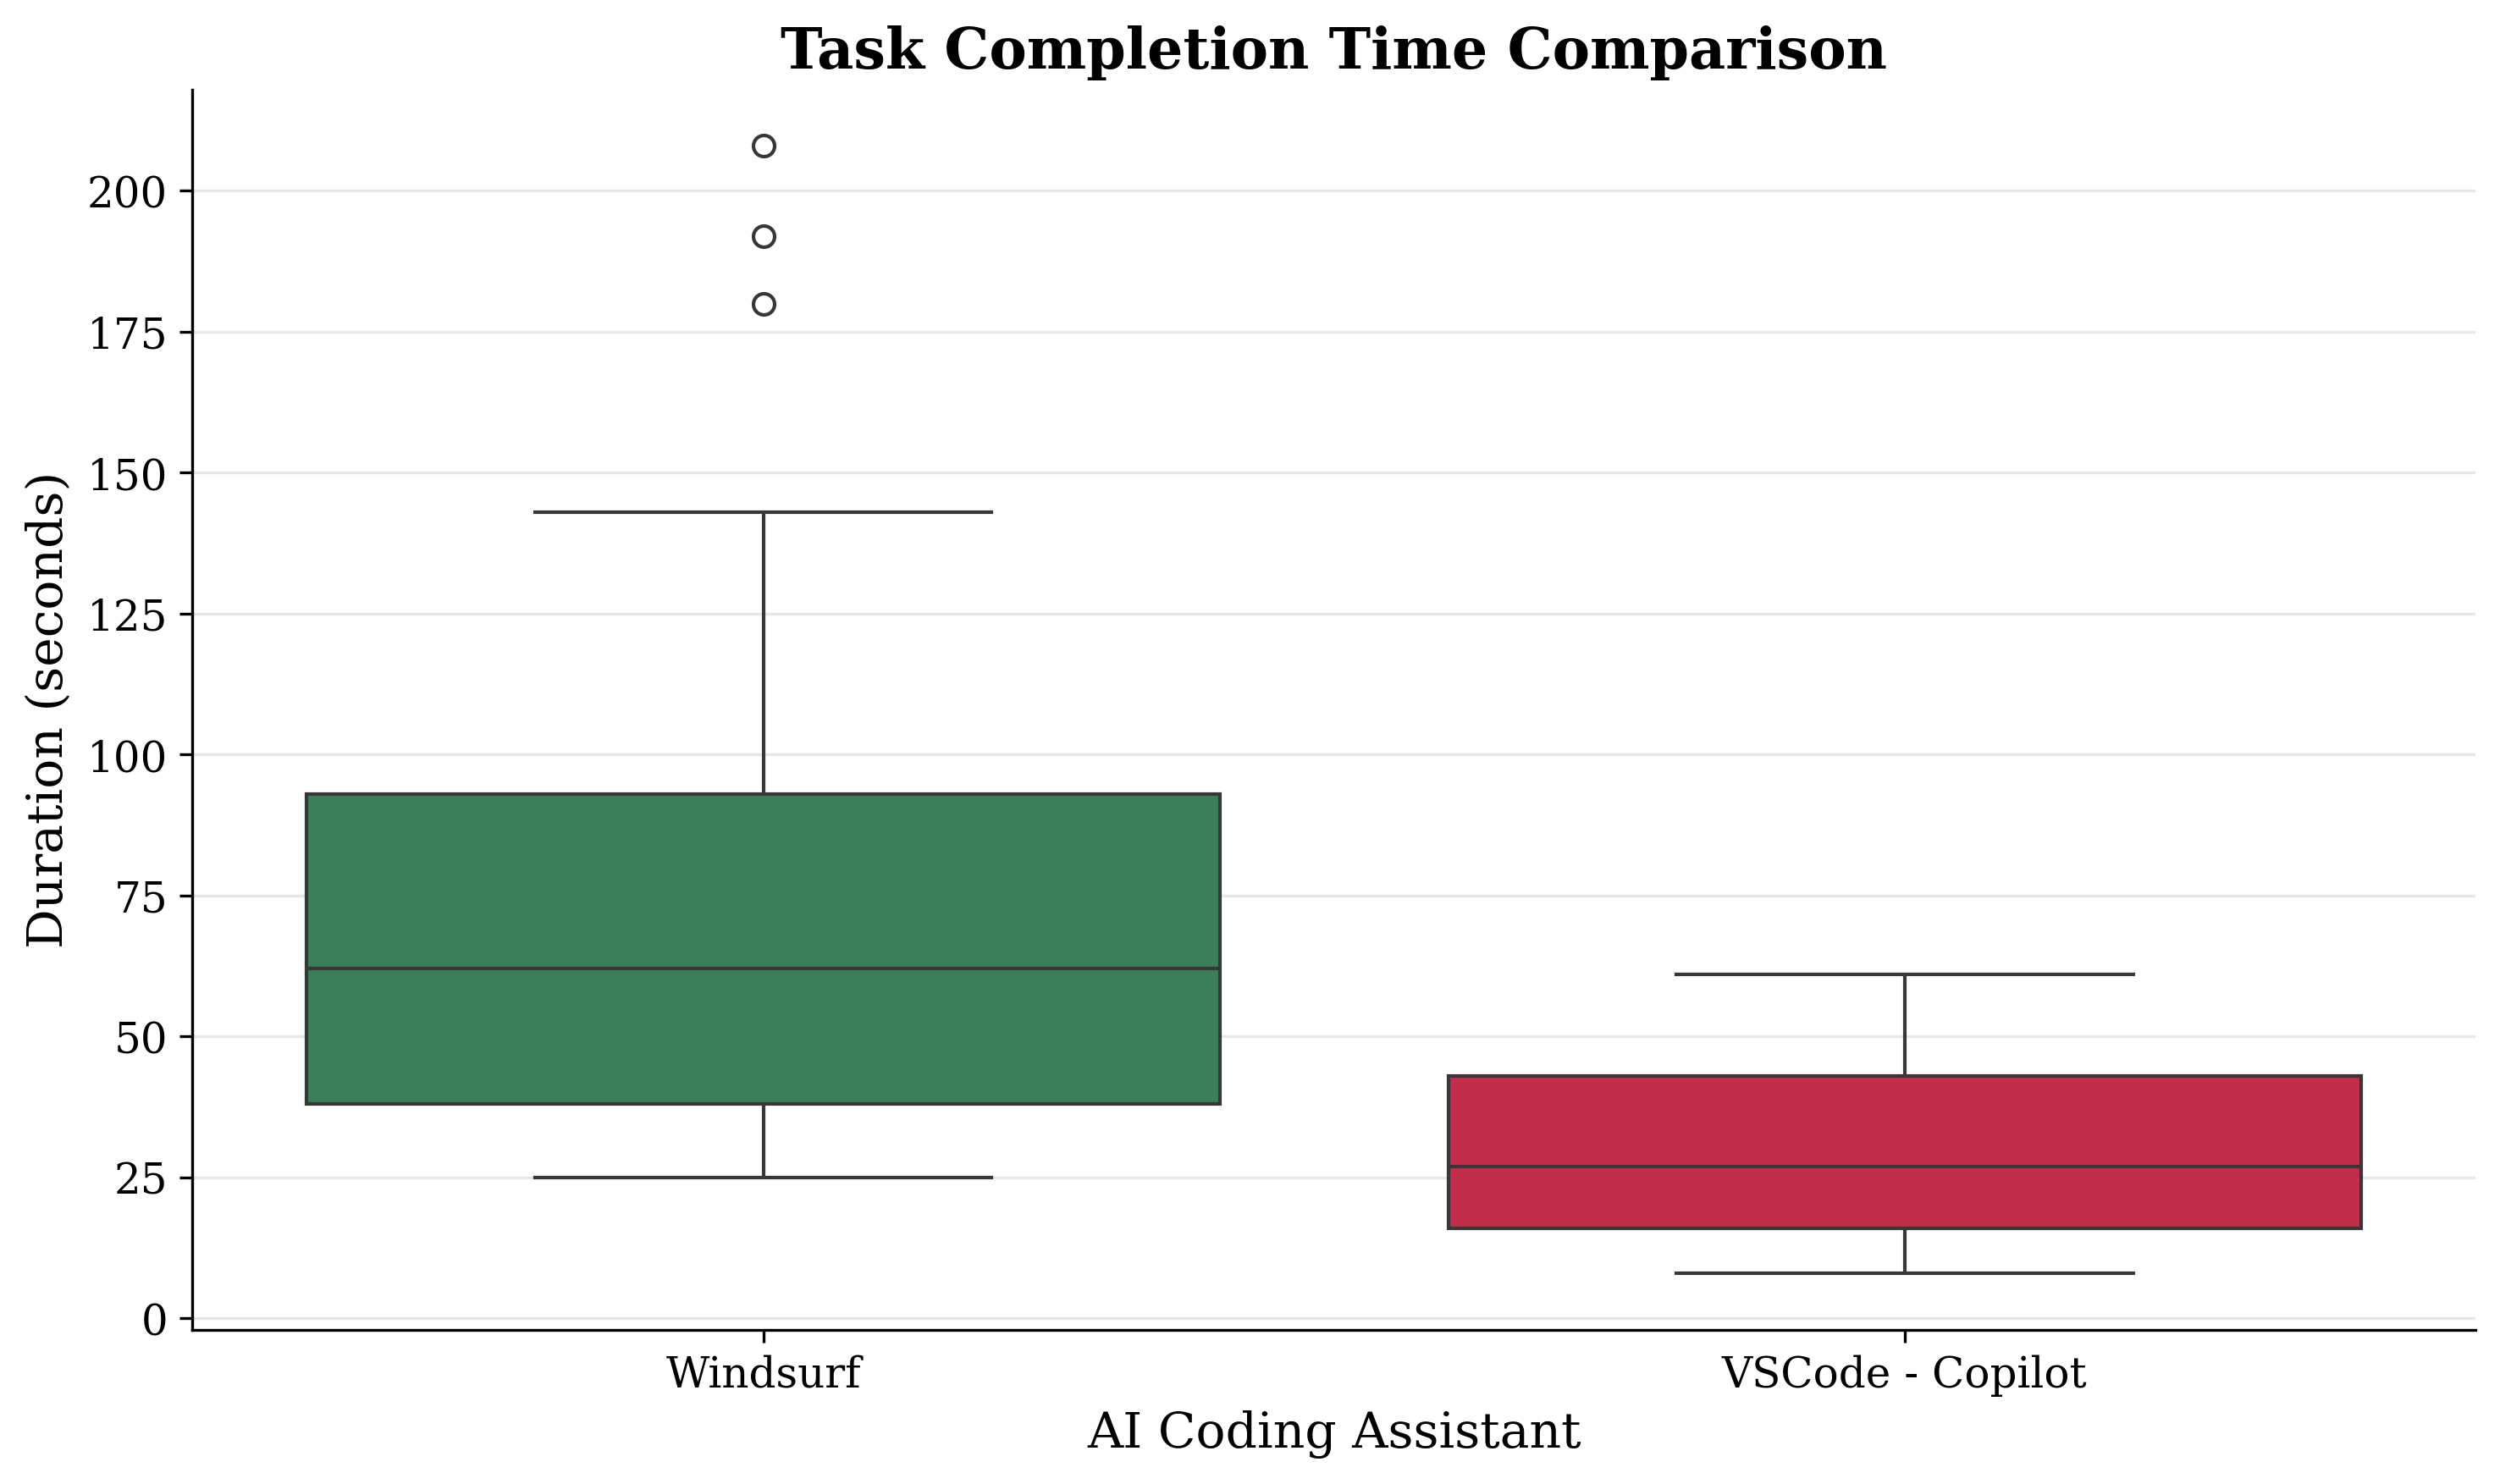
\includegraphics[width=1\linewidth]{images/4_duration_comparison.png}
  \caption{Compared the execution speed across all executions of Windsurf Cascade and Github Copilot}
  \label{fig:runtime-comparison}
\end{figure}


Figure \ref{fig:runtime-comparison} shows a comparison of the average execution speed and distribution of the systems across all executed prompts and iterations. Windsurf Cascade achieved an average speed of 75.1 seconds, while Github Copilot via VSCode achieved an average execution speed of 29.2 seconds. Github Copilot remains very consistent across all executions, while Windsurf Cascade achieved large fluctuations in execution speed. The longest execution time achieved by Windsurf was 208 seconds for the prompt ''C1'' in run two.

\begin{figure}[htbp]
  \centering
  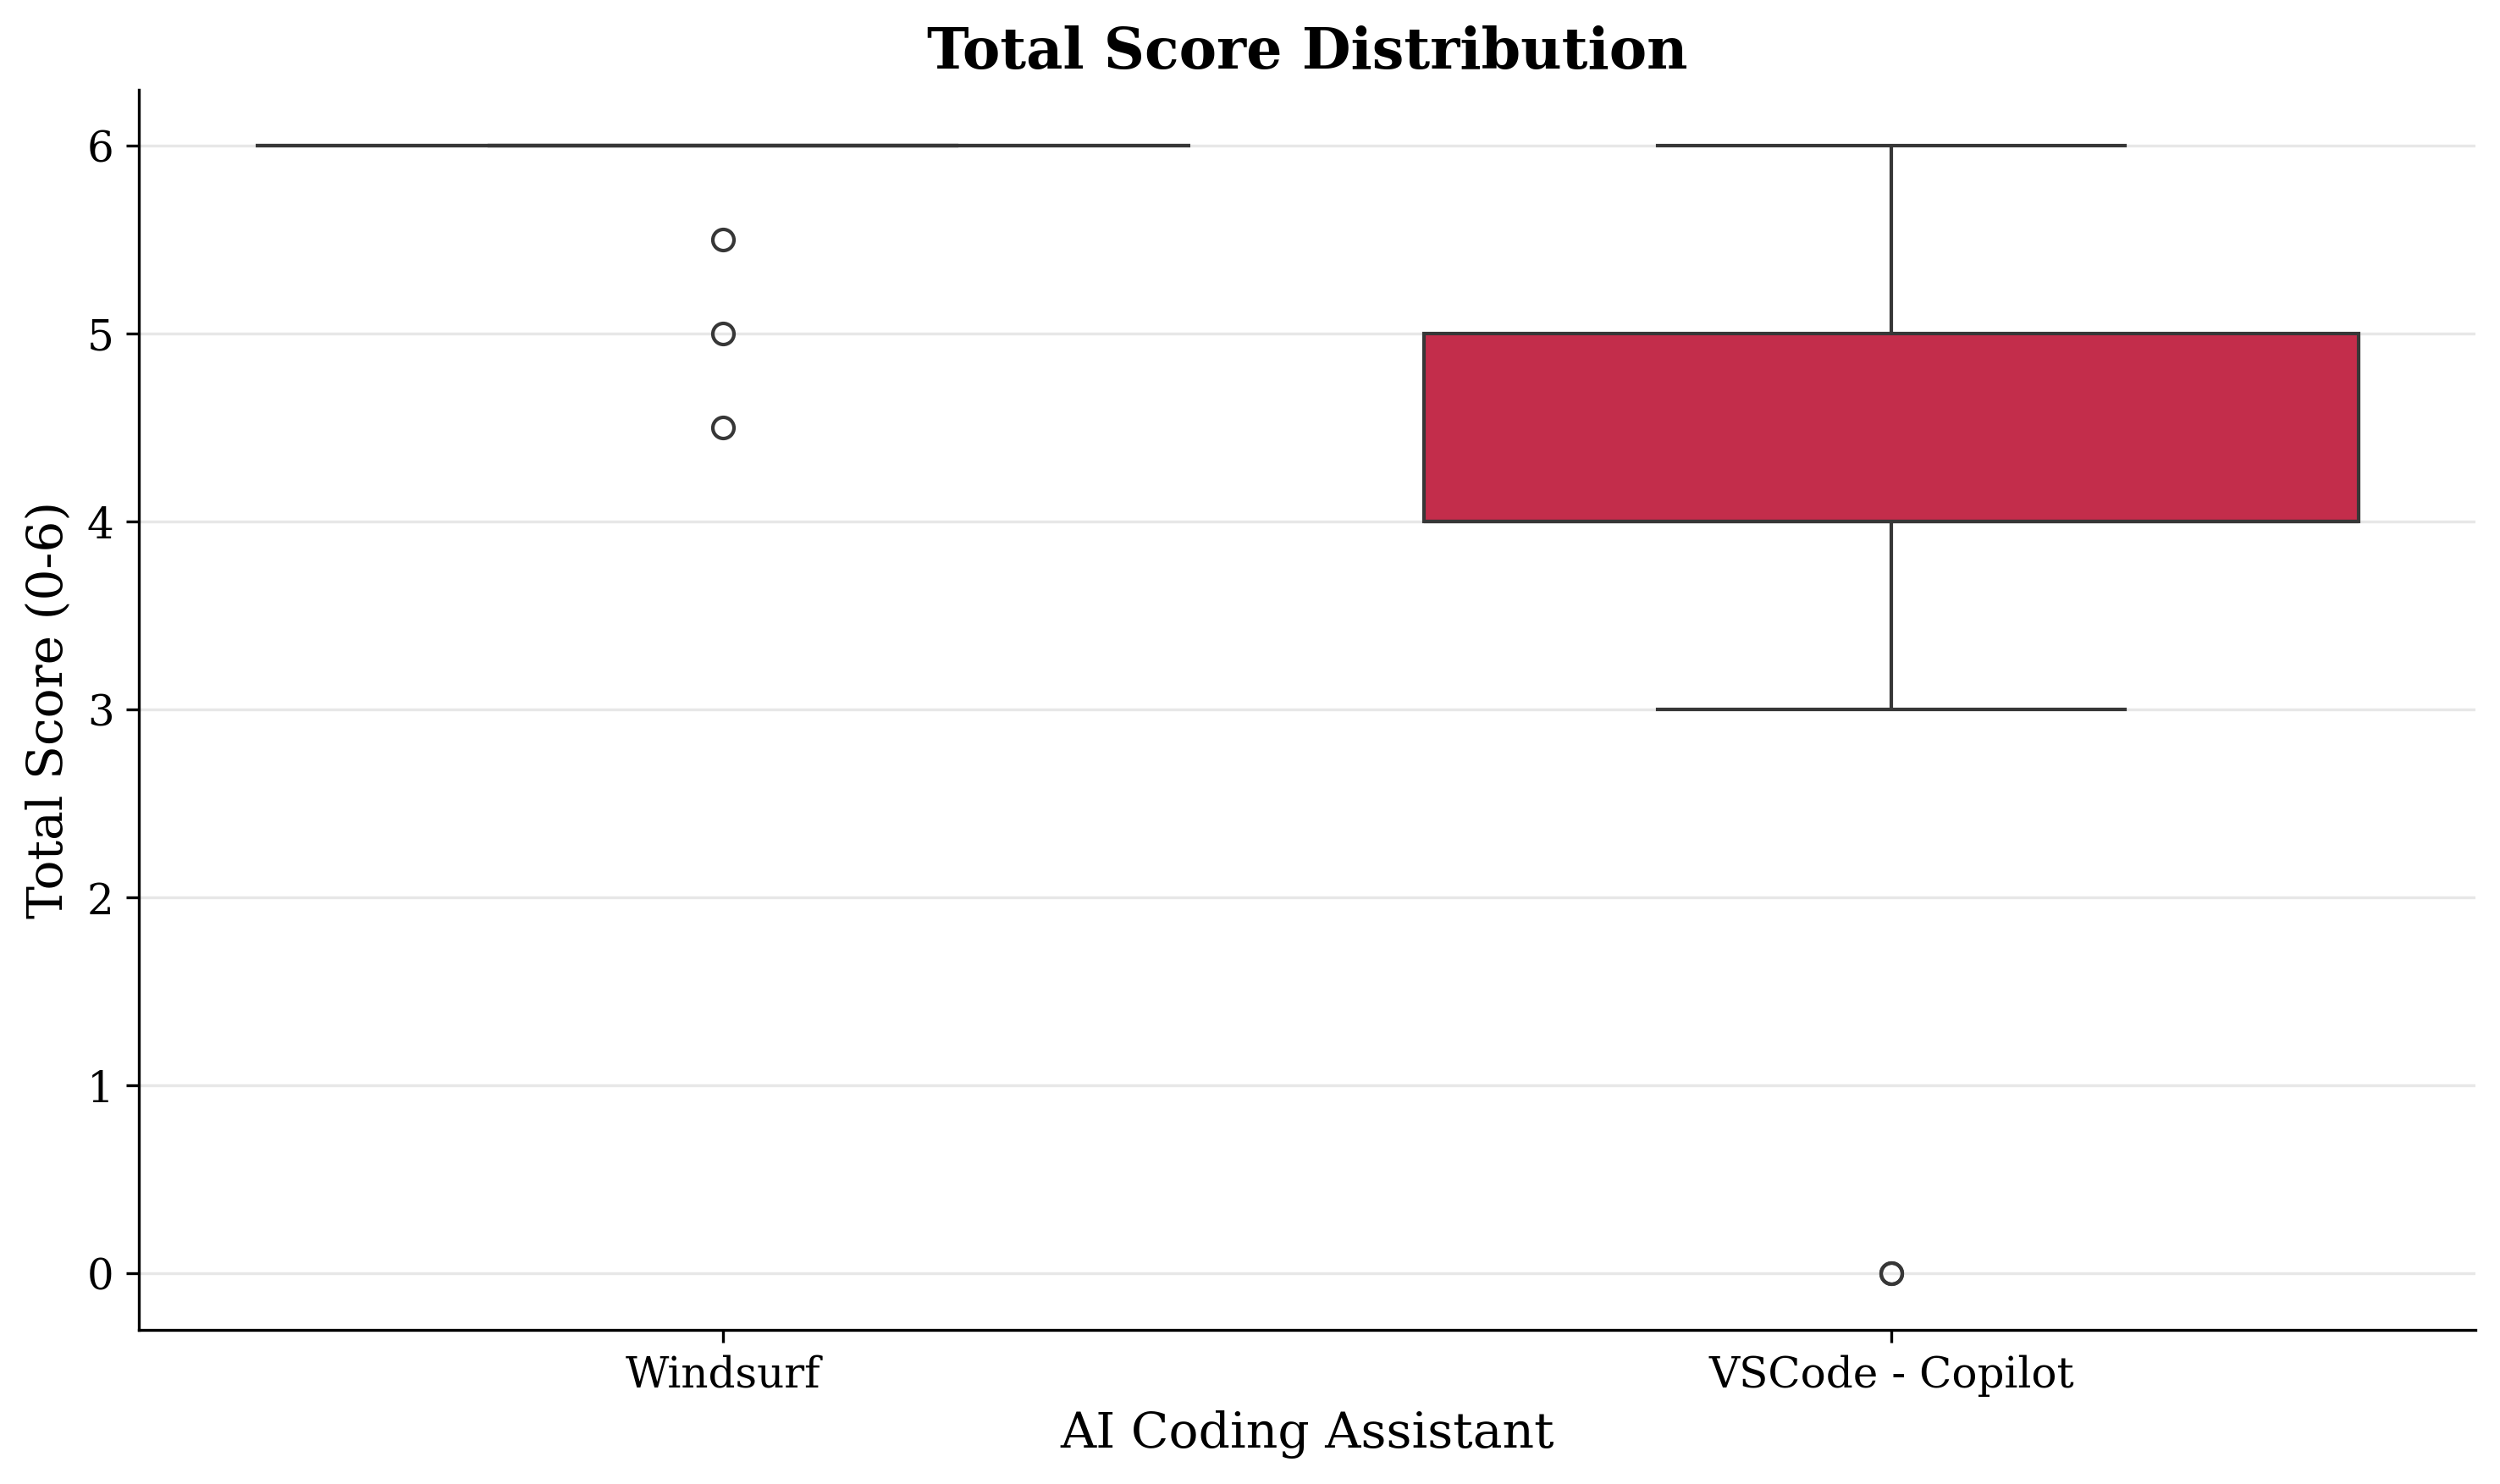
\includegraphics[width=1\linewidth]{images/2_score_distribution.png}
  \caption{Compared the total score distribution across all executions of Windsurf Cascade and Github Copilot}
  \label{fig:score-distribution}
\end{figure}


Figure \ref{fig:score-distribution} shows the average distribution of points for each system across all tasks and runs. Windsurf Cascade achieved an average score of 5.91 points with a standard deviation $\sigma$ of 0.32 points. Github Copilot achieved an average score of 4.06 points with a standard deviation $\sigma$ of 1.35 points. 


\begin{figure}[htbp]
  \centering
  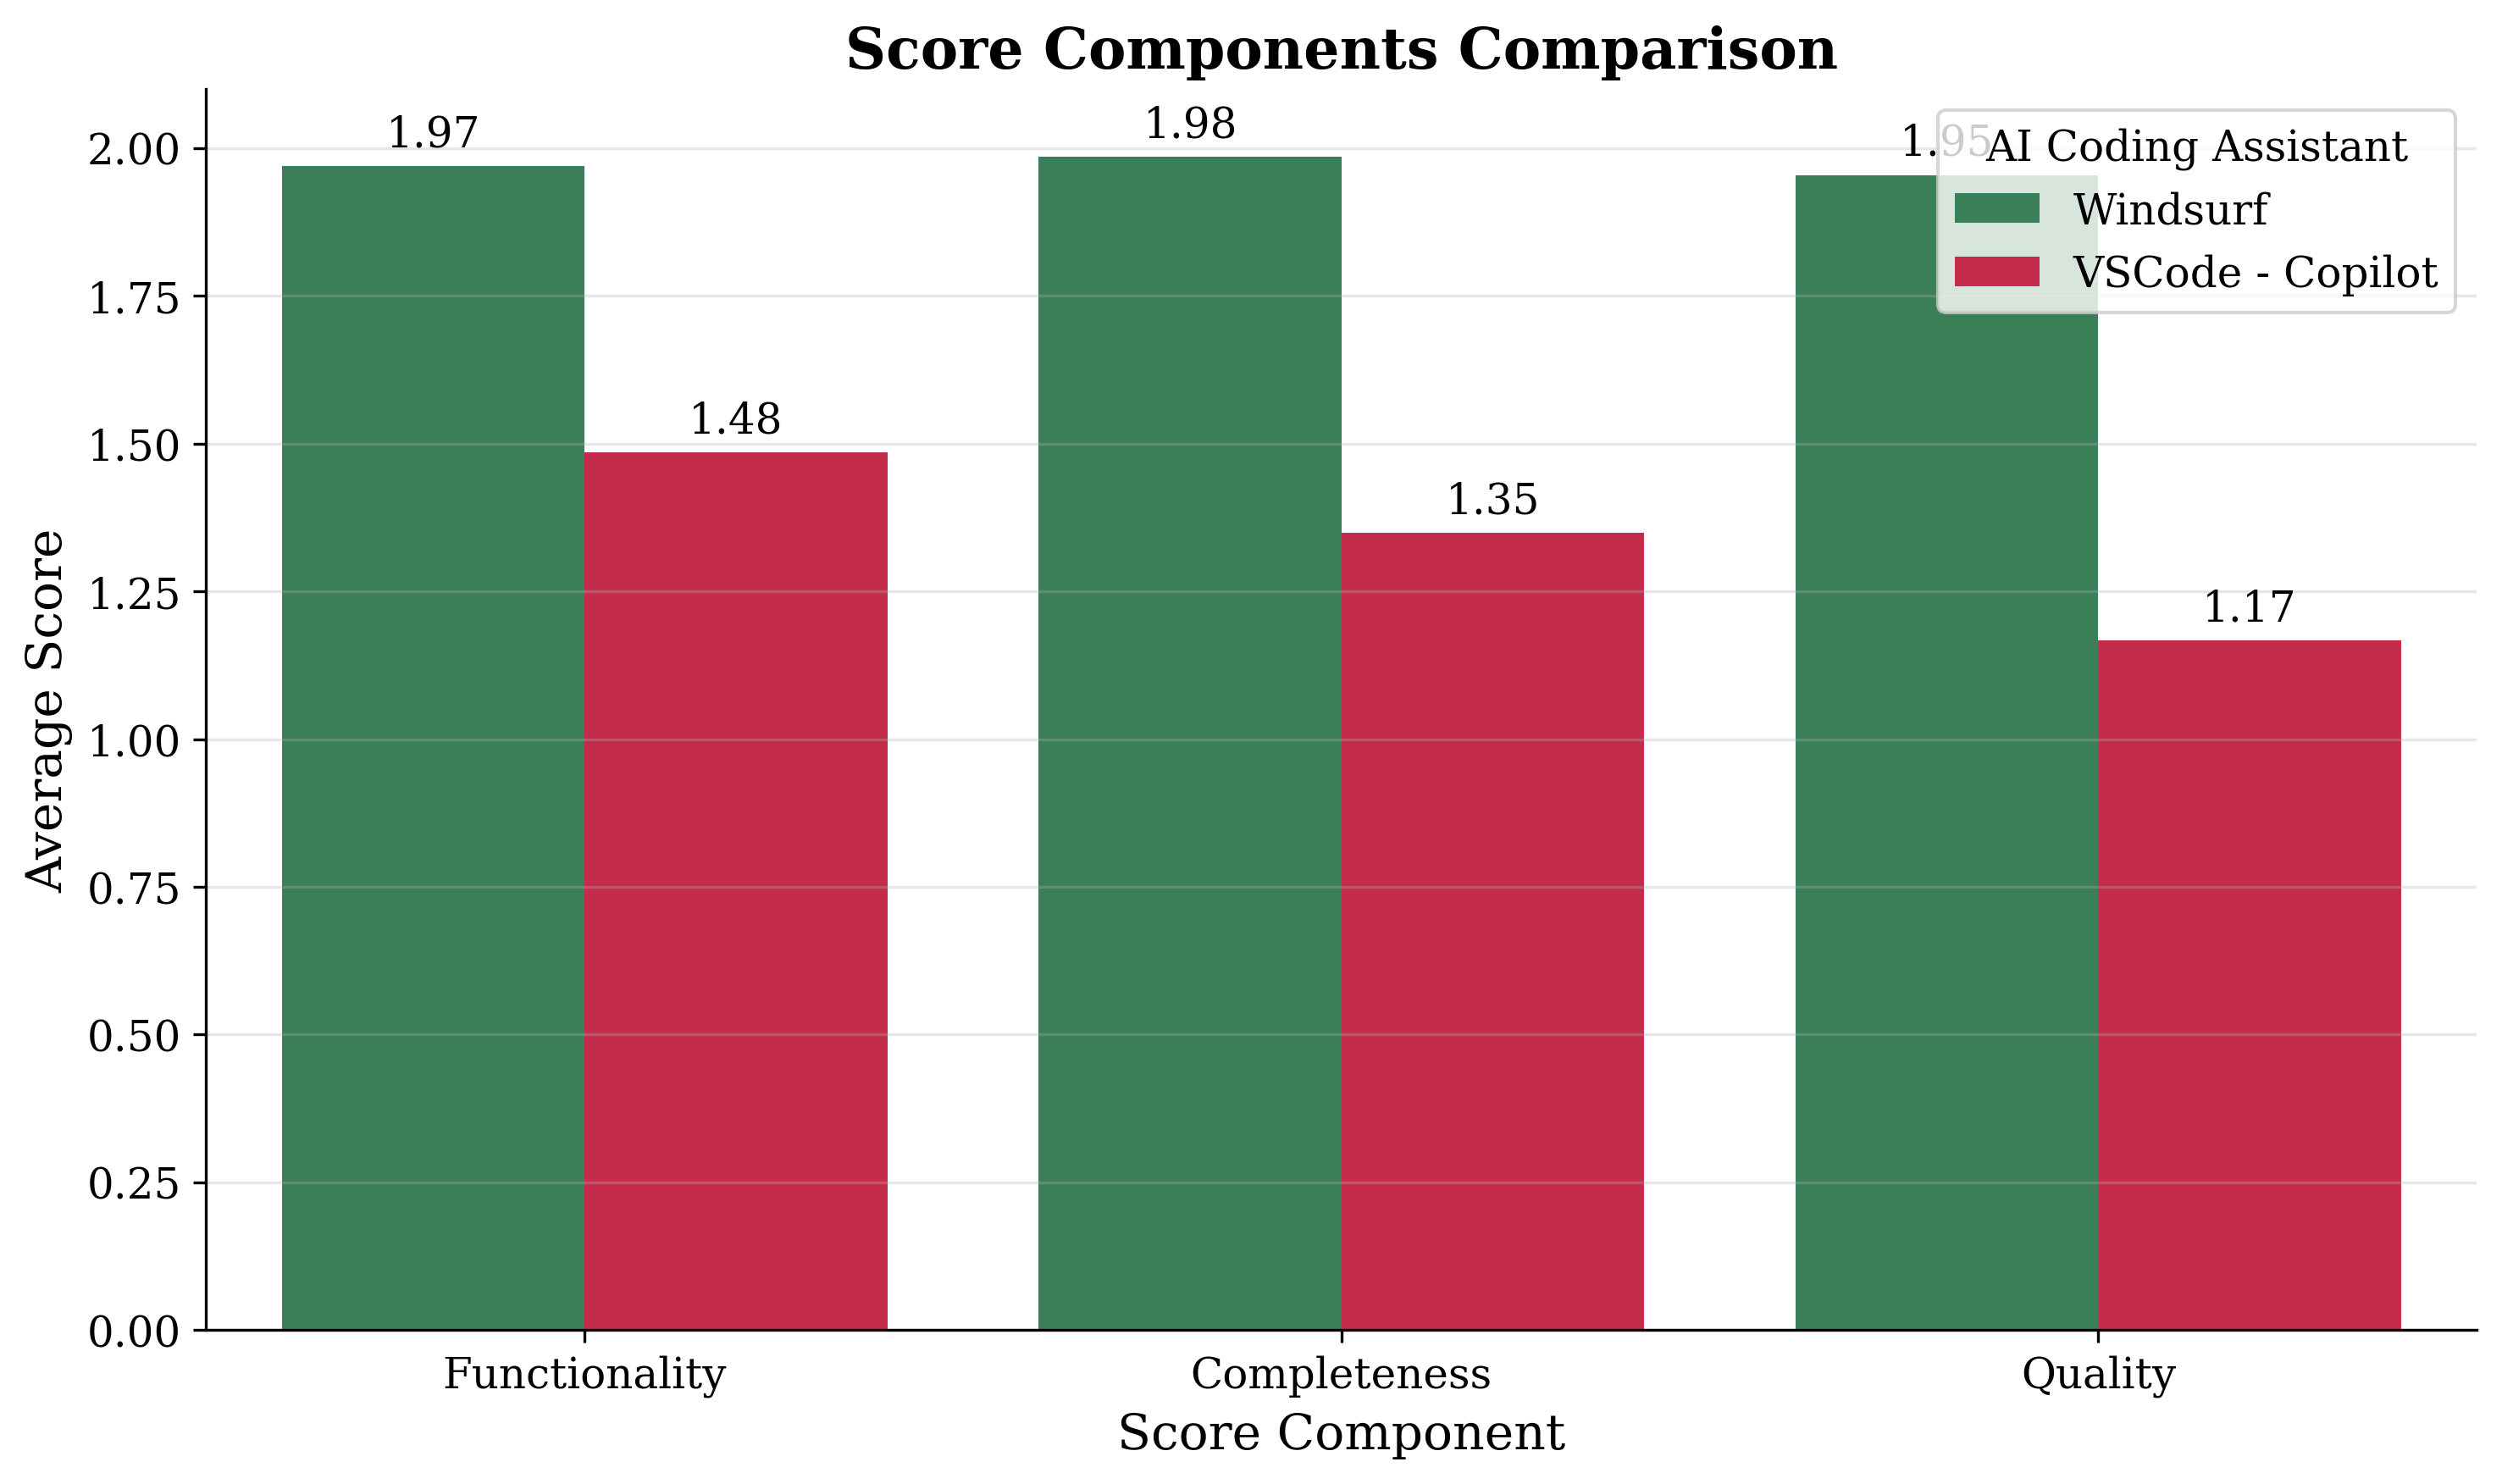
\includegraphics[width=1\linewidth]{images/5_score_components.png}
  \caption{Compared the score components of all executions of Windsurf Cascade and Github Copilot}
  \label{fig:score-components}
\end{figure}

Figure \ref{fig:score-components} shows a comparison of Windsurf Cascade and Github Copilot via VSCode according to the three evaluation criteria or components of the evaluation. The graph shows the average scores of the respective systems across all runs based on the criteria of quality, functionality and completeness. Windsurf Cascade achieved an average score of 1.97 out of 2 points for functionality. Windsurf Cascade achieved an average score of 1.98 out of 2 points for completeness and an average score of 1.95 out of 2 points for quality. Github Copilot via VSCode, on the other hand, achieved an average score of 1.48 out of 2 points for functionality, an average score of 1.35 points for completeness and a score of 1.17 out of 2 points for quality.


\begin{figure}[htbp]
  \centering
  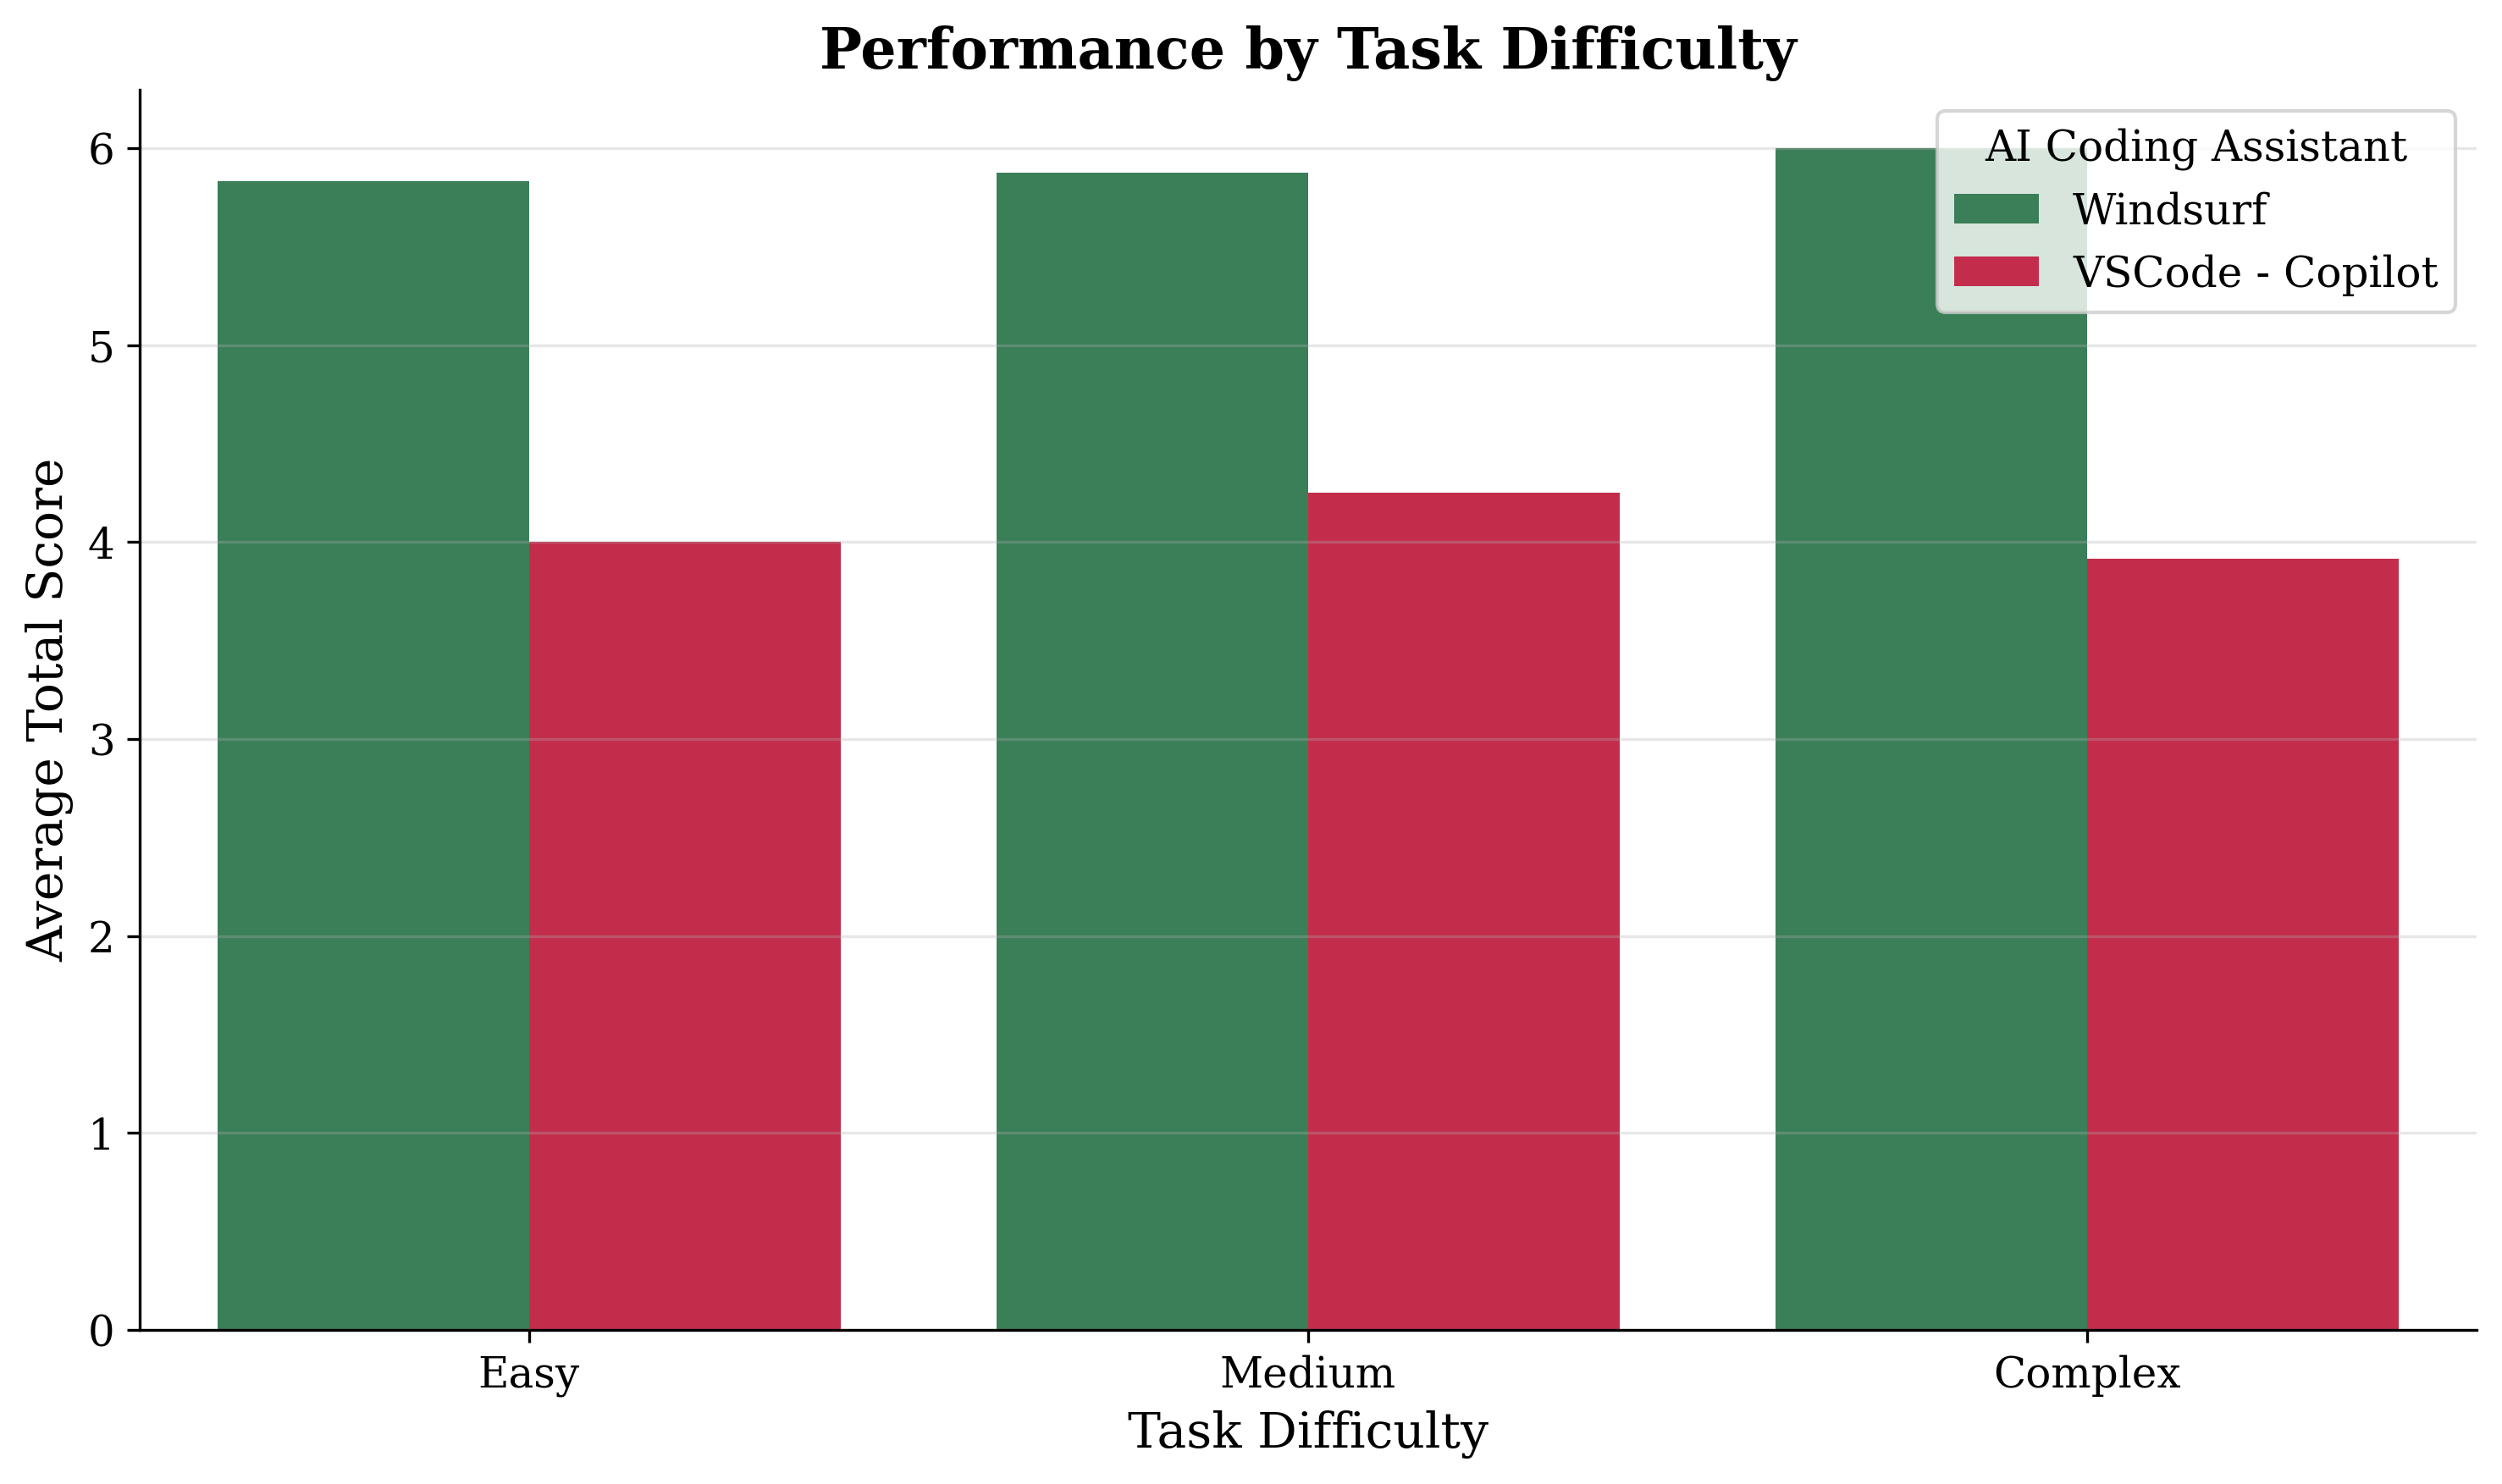
\includegraphics[width=1\linewidth]{images/3_difficulty_performance.png}
  \caption{Compared the performance by task difficulty of all executions of Windsurf Cascade and Github Copilot}
  \label{fig:performance-tasks}
\end{figure}

Figure \ref{fig:performance-tasks} shows the average score of the systems based on the three categories easy, medium and complex and compares the two systems with each other in these respects. In the easy category, Windsurf achieved an average score of 5.83 out of 6 points, in the medium category 5.88 out of 6 points and in the complex tasks the maximum score of 6 out of 6 points. Github Copilot achieved an average score of 4 out of 6 points in the easy category, 4.25 out of 6 points in the medium category prompts, and an average score of 3.92 out of 6 points in the complex tasks.


\begin{figure}[htbp]
  \centering
  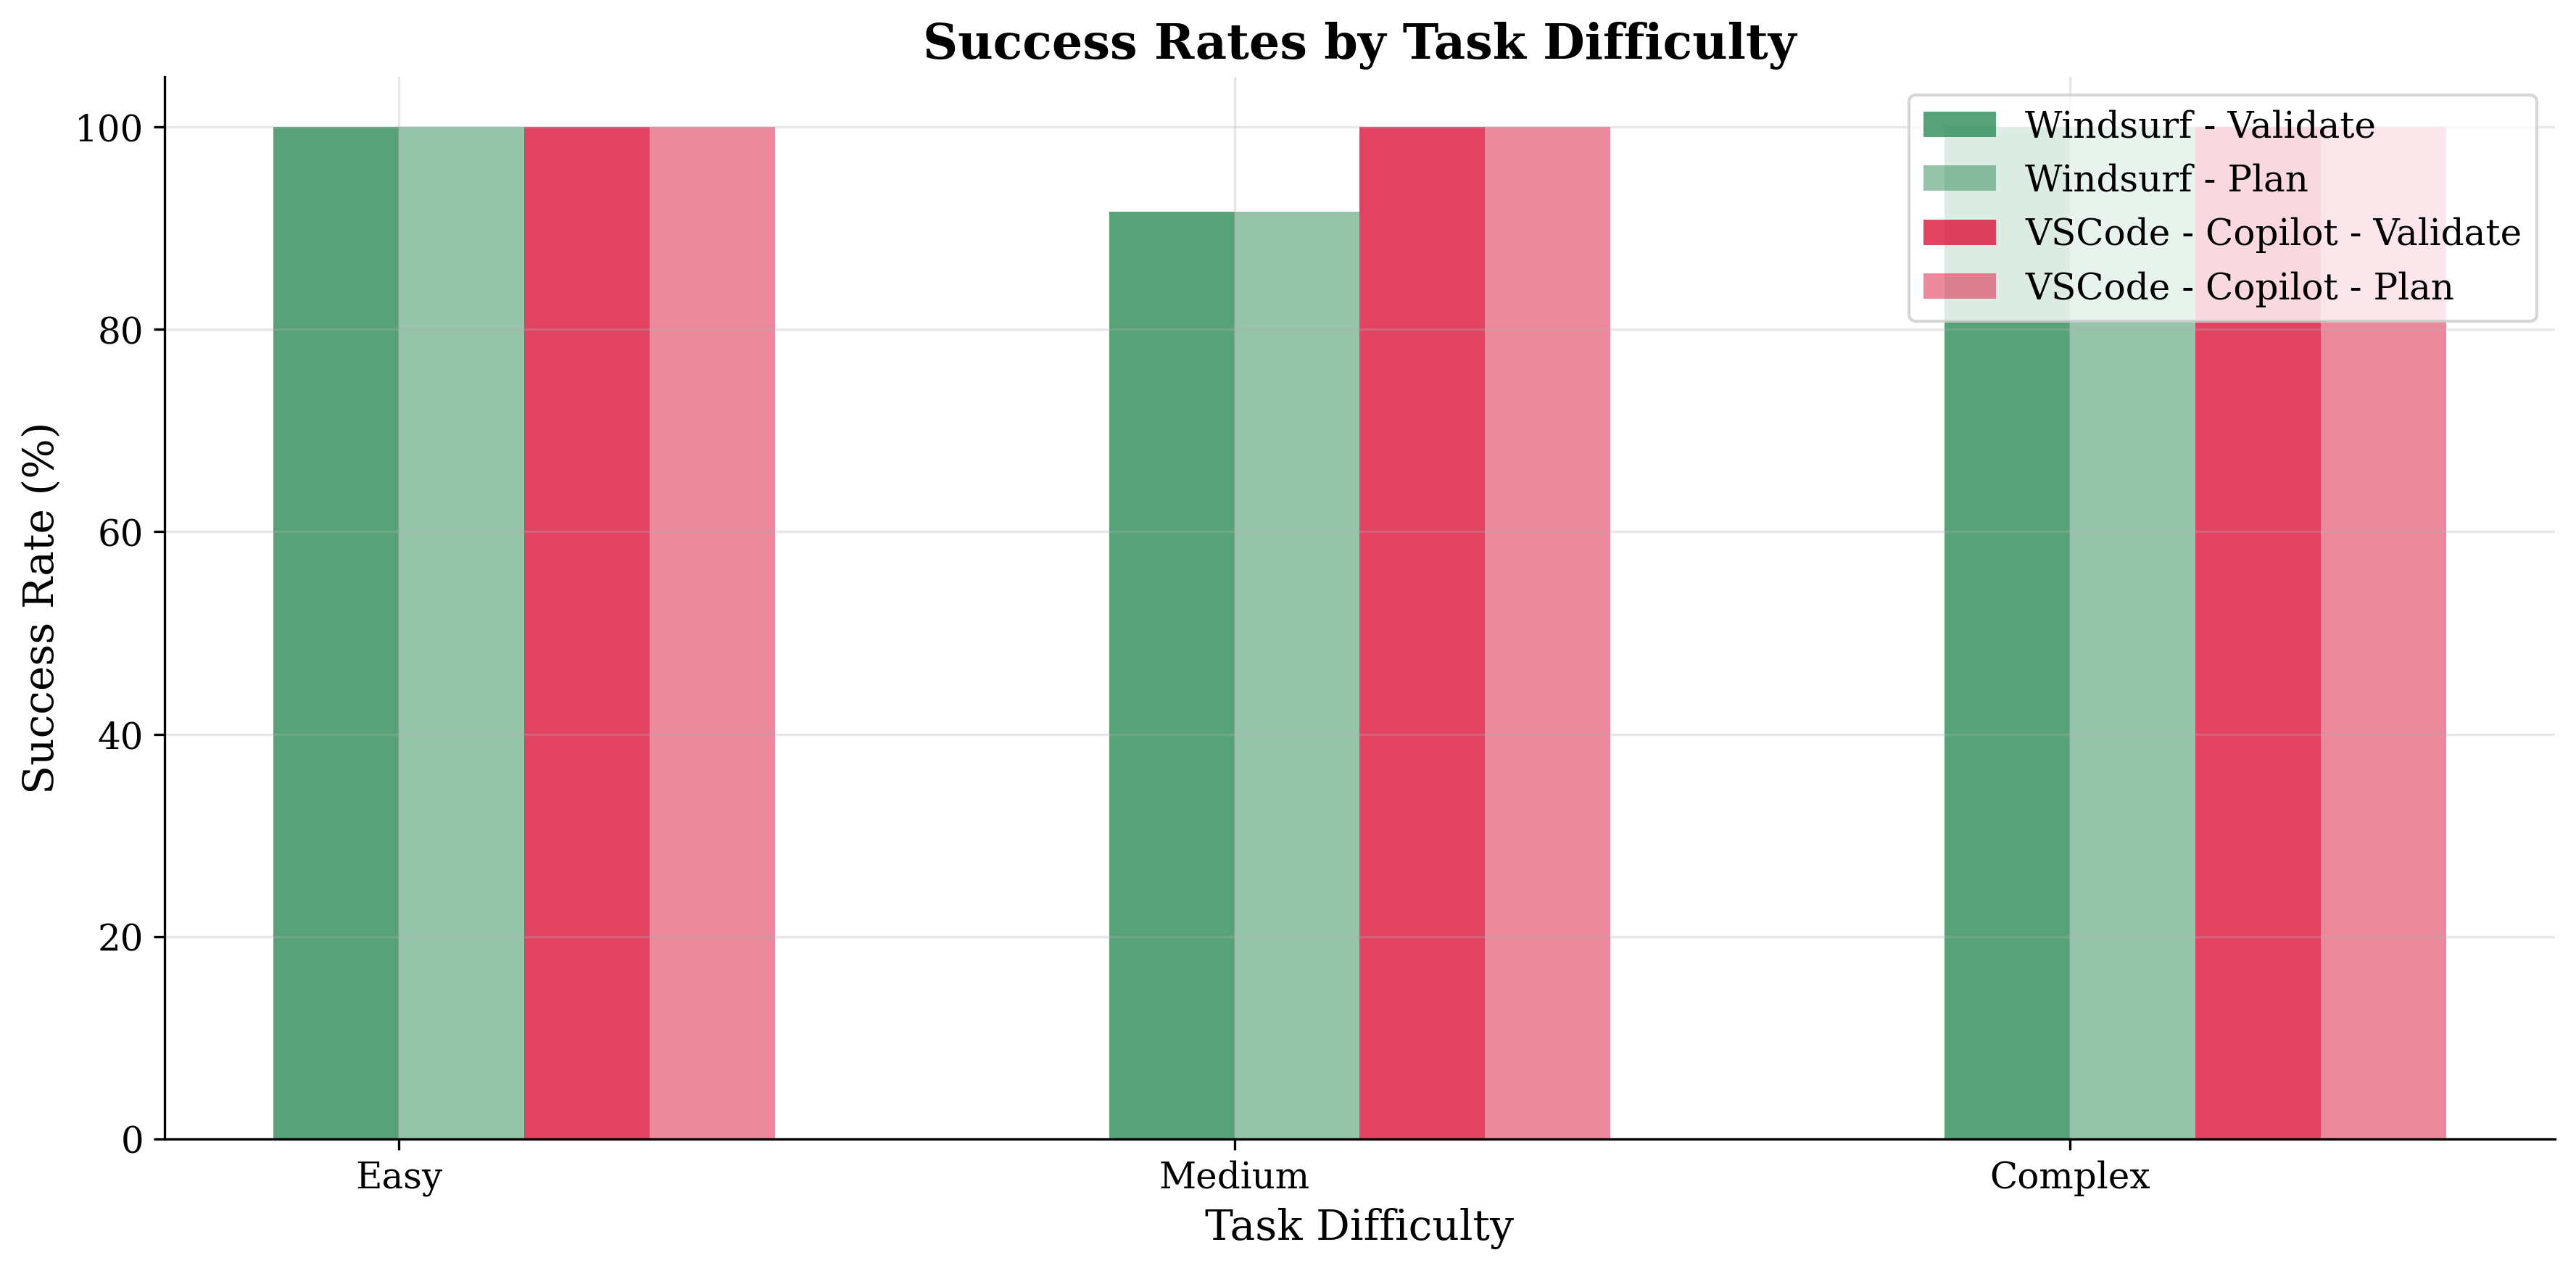
\includegraphics[width=1\linewidth]{images/7_success_by_difficulty.png}
  \caption{Compared the success of the validate and plan operation across all executions of Windsurf Cascade and Github Copilot}
  \label{fig:operation-success}
\end{figure}

Figure \ref{fig:operation-success} shows the success rates of the evaluation commands ''terraform validate'' and ''terraform plan'' executed after each evaluation of a prompt. Overall, Windsurfe Cascade achieved a success rate of 97\%, while Github copilot achieved a success rate of 100\% over both operations and all executions.

\section{Discussion}
\label{sec:discussion}

The aim of this work was to compare the usefulness and quality of the two AI programming aids Windsurf Cascade and Github Copilot and to relate them to quality in general. This section deals with the interpretation of the results presented in the last section.

Starting with the average speed of code and response generation for the two AI programming aids. Copilot shows significantly faster performance than Windsurf overall, with Github Copilot's responses and generation being 61.1\% faster than Windsurf's response generation. This significant difference in speed can also be attributed in part to the quality of the responses. Windsurf achieves an almost flawless quality rating across all iterations and runs, while Copilot achieves an average rating that is 31.3\% below the quality of Windsurf. This means that the Github Copilot responses in this evaluation are almost a third worse than the responses generated by Windsurf Cascade. Also noteworthy is the standard deviation mentioned above, which is 0.32 points for Windsurf and 1.35 points for Copilot, allowing conclusions to be drawn about the reliability and consistency of the responses from the two systems. In comparison, Windsurf achieves an answer rate that is almost three times more consistent than Copilot. This shows that even with different types and kinds of tasks, the procedure used by Windsurf Cascade is best equipped and provides consistent answers even for complex tasks. With Copilot, on the other hand, it seems as if the model behind it does not receive sufficiently structured information and is unable to provide consistent answers.


The reason for these results can be better understood by looking at the results of the evaluation of the individual score components. Here, Copilot shows significant problems in generating quality code, i.e. the system pays attention to best practices in Terraform programming or the use of variables and configuration files. In this category, Copilot 1.17 received an average score of 2 out of 2 possible points, meaning that just over half of the possible best practices or code quality were achieved and generated in the responses and code generated by GitHub Copilot. This can be attributed to the fact that Windsurf Cascade demonstrably assumes that the system should be ready for production after generation, while Copilot pays attention to executing the specified requirements, but does not do anything beyond what is described. This can also be attributed to the high variance in responses, as different iterations of the input prompts can be interpreted differently and no attempt is made to truly understand the entire system or the thinking behind it.

However, due to the increased complexity of the tasks generated by Windsurf, this system is also more prone to problems or potential errors. For example, in 4 out of 33 cases, it was not possible to automatically insert the generated code in Windsurf, and the code had to be entered manually into the files. With Github Copilot, on the other hand, only 2 out of 33 cases were not possible, and this behavior only occurred with Copilot for complex tasks, whereas with Windsurf it occurred in all categories. In addition, the execution of the validation and planning steps with Windsurf was not successful in one out of 33 cases. Furthermore, Copilot does not generate any code at all in two consecutive executions for the task category ''Complex'' with the prompt ''C2'' once again illustrating that Copilot quickly reaches its limits when it comes to a specific type of tasks. 

The results described imply that although the generation time of Windsurf Cascade is significantly longer, the quality of the results speaks for itself. The system achieves an almost flawless result with Terraform and is the clearly better choice for Terraform code generation under the conditions described. However, caution is advised, as this study only analyses a specific part of AI programming systems and does not deal with the agent mode of the two systems or with models other than Claude Sonnet 4, with which different systems may interact better or worse. Furthermore, the evaluation is not intended to suggest that Github Copilot is a poor tool, but rather that Windsurf achieves significantly more consistent and better results than Copilot under the given circumstances and is therefore more useful for experienced and inexperienced developers under the conditions described, as the quality and reliability of the results are higher and more meaningful.
\section{Conclusion}
\label{sec:conclusion}

The results of the study show that AI programming aids are perfectly capable of performing simple to complex tasks and can also provide strong support for developers and newcomers in the field of IaC. Even though there are significant differences in the quality of the output and generated responses, both tools examined demonstrate the ability to solve complex tasks and generate clean, structured and well-founded Terraform, thereby meeting the user's requirements. Nevertheless, Windsurf proves to be a more robust tool that is better suited to this use case in terms of output quality. As a result, it is advisable to use Windsurf when programming IaC with Terraform. However, this study only evaluated Windsurf Cascade and Github Copilot via VSCode and did not consider other systems such as Cursor. The next logical step would therefore be to conduct an expanded study with all major players in the AI programming tools field, using different modes and not limiting ourselves to just ‘edit’ or ‘chat’ mode, but also modes such as agent mode, which is becoming increasingly popular. The tools should also be tested with difficult tasks using existing codebases in order to examine how successfully the tools adapt to existing coding styles.

% Acknowledgments
\section*{Acknowledgments}
This work was conducted independently. The author used Windsurf Cascade and GitHub Copilot via VisualSudioCode for the IaC evaluation and DeepL for language assistance.

\appendix
\section{Supplementary Materials}
The code, results and experimental configurations used in this study are available at: \\
\url{https://github.com/L4XB/terraform-ai-study}

% Bibliography
\bibliographystyle{ACM-Reference-Format}
\bibliography{references}

% Balance columns
\balance



\end{document}





